% !TEX root =  ICRA2012-Patil.tex

We present simulation results for two scenarios: (1) a car-like robot with second order dynamics, and (2) a nonholonomic bevel-tip flexible needle, with stochastic dynamics and partial and noisy sensing feedback. In each case, we initialize our method with a nominal plan computed using an RRT planner \cite{Book:LaValle06}. We tested our C++ implementation on a 3.33 GHz Intel\textsuperscript{\tiny \textregistered} i7\textsuperscript{\tiny TM} PC. %We empirically demonstrate that our method provides a more accurate estimation of the \emph{a priori} probability distributions of the robot state and the probability of collision compared to prior methods.

We validate our method by comparing the estimated collision probability with the ground truth probability computed using a million Monte Carlo simulations (considered as ground truth) of the given motion plan and counting the ratio of collision free simulations. Each execution is simulated in a closed-loop fashion using the given linear feedback controller and a Kalman filter, and with artificially generated motion and measurement noise.

\subsection{Car-like Robot with Second Order Dynamics}

We consider a nonholonomic car-like robot with second order dynamics, navigating in a 2D environment with obstacles (Fig.\ \ref{fig:car2d}). The state of the robot, $\mathbf{x} = [x, y, \theta, v]^T \in \mathbb{R}^4$, consists of its position $[x, y]$, its orientation $\theta$, and its speed $v$. The control input $\mathbf{u} = [a, \phi]^T \in \mathbb{R}^2$, consists of the acceleration $a$, and steering angle $\phi$, corrupted by motion noise $\mathbf{m} = [\tilde{a}, \tilde{\phi}]^T \sim \mathcal{N}[\mathbf{0}, M]$. This gives the following stochastic dynamics model:
\begin{equation}
\mathbf{f}[\mathbf{x}, \mathbf{u}, \mathbf{m}] = \begin{bmatrix} x + \tau v \cos\theta \\ y + \tau v \sin \theta \\ \theta + \tau v \tan(\phi + \tilde{\phi})/d \\ v + \tau(a + \tilde{a}) \end{bmatrix},
\end{equation}
where $\tau$ is the time step, and $d$ is the length of the car.

The robot localizes itself using noisy signal measurements from two beacons $b_1$ and $b_2$, placed in the environment at locations $[\check{x}_1, \check{y}_1]$ and $[\check{x}_2, \check{y}_2]$ respectively. The strength of the signal decays quadratically with the distance to the beacon. The robot also measures its current speed using an on-board speedometer. %The observation vector $\mathbf{z} \in \mathbb{R}^3$, consists of two readings of signal strengths from the beacons and a speed measurement from the speedometer, corrupted by sensing noise $\mathbf{n} \sim \mathcal{N}[\mathbf{0}, N]$.
This gives us the following stochastic measurement model:
\begin{equation}
\mathbf{h}[\mathbf{x}, \mathbf{n}] = \begin{bmatrix} 1/((x - \check{x}_1)^2 + (y - \check{y}_1)^2 + 1) \\ 1/((x - \check{x}_2)^2 + (y - \check{y}_2)^2 + 1) \\ v \end{bmatrix} + \mathbf{n}.
\end{equation}
where the observation vector $\mathbf{z} \in \mathbb{R}^3$, consists of two readings of signal strengths from the beacons and a speed measurement, corrupted by sensing noise $\mathbf{n} \sim \mathcal{N}[\mathbf{0}, N]$.

Fig.\ \ref{fig:1b} shows the discrepancy between the unconditional and conditional distributions in the presence of obstacles. The conditional distributions computed using our method provide an accurate estimate of the distribution of the collision free robot states along the plan, thus providing an accurate estimate of the probability of collision. Fig.\ \ref{fig:1c} shows how the mean of the conditional distribution can deviate significantly in the close vicinity of obstacles. Interestingly, the conditional and unconditional distributions become identical towards the end of the plan in the absence of obstacles.

\subsection{Nonholonomic Bevel-tip Flexible Needle}

\begin{figure*}[!t]
{\,} \hfill
%\subfigure[\label{fig:2a}]{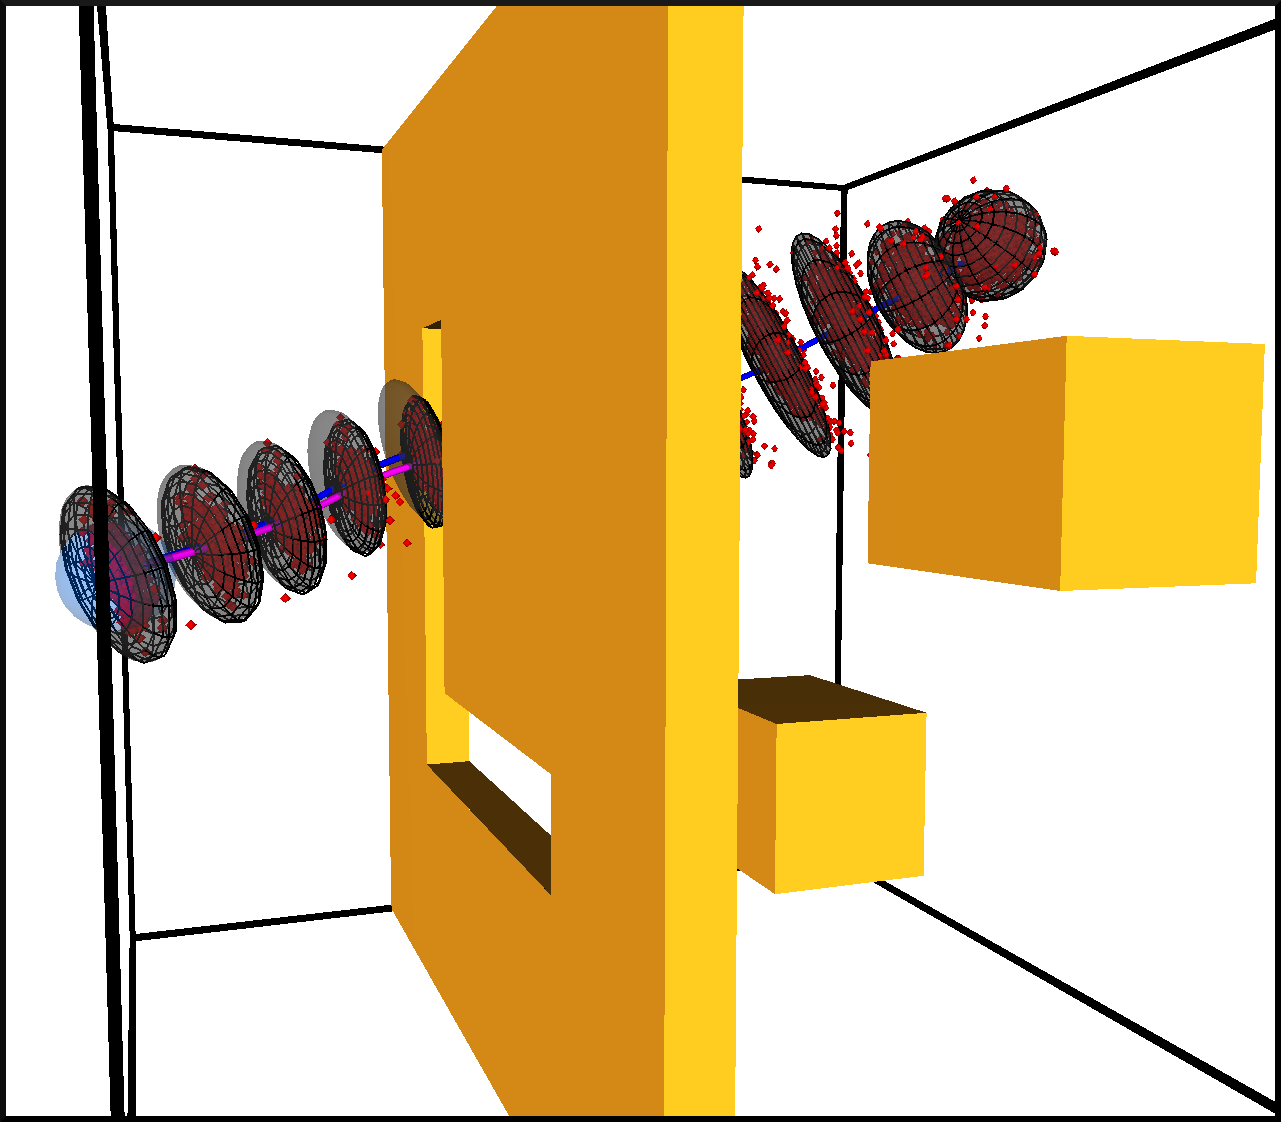
\includegraphics[width=160pt,clip]{figures/needle3d/plan1.png}}
\subfigure[3D test case \label{fig:2a}]{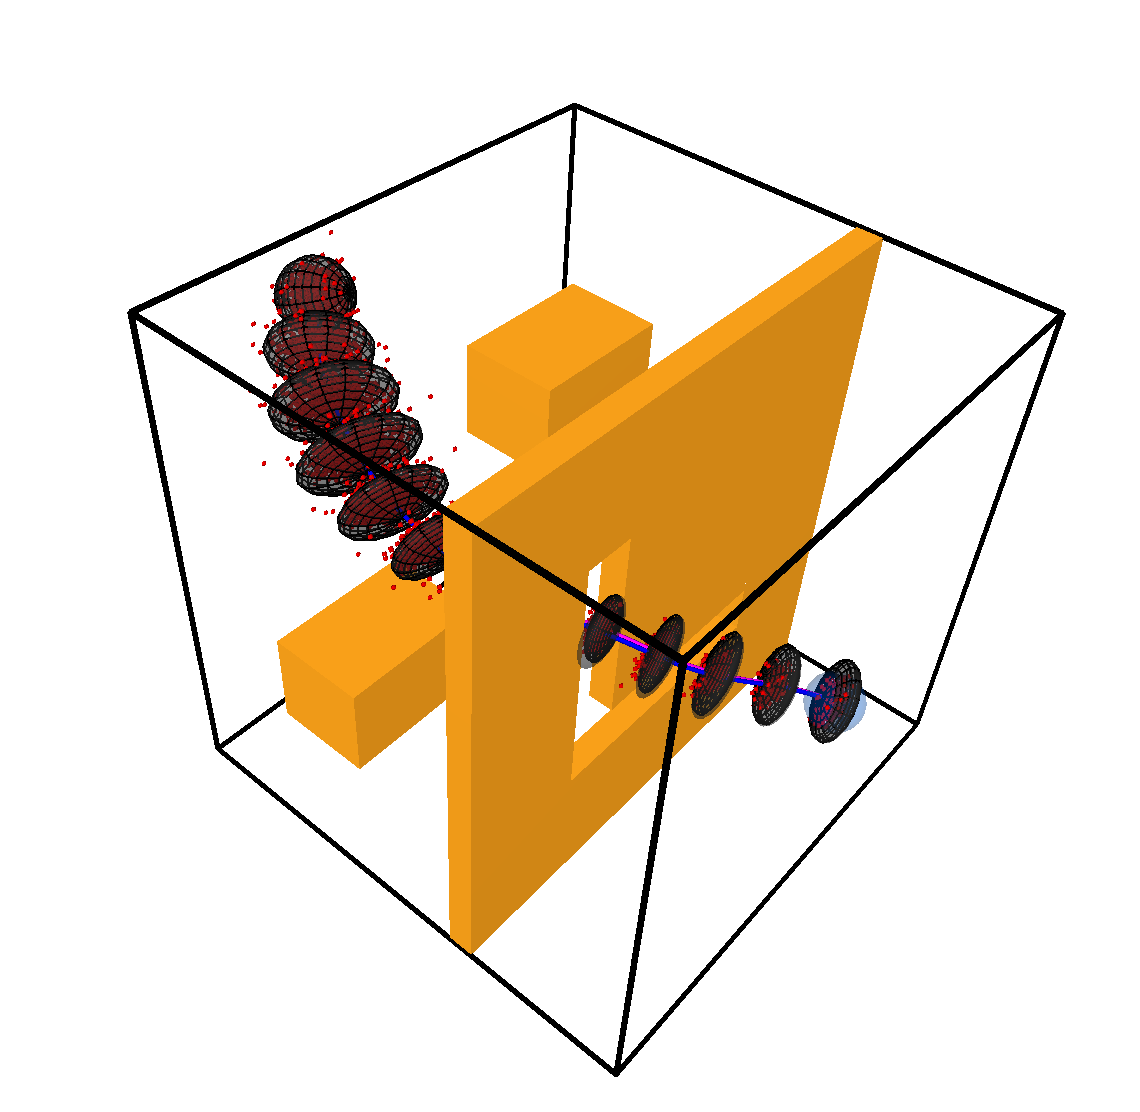
\includegraphics[trim=0pt 30pt 0pt 0pt, clip, width=100pt,clip]{figures/needle3d/plan1-top.png}}
\hfill
\subfigure[Zoom into narrow corridor\label{fig:2b}]{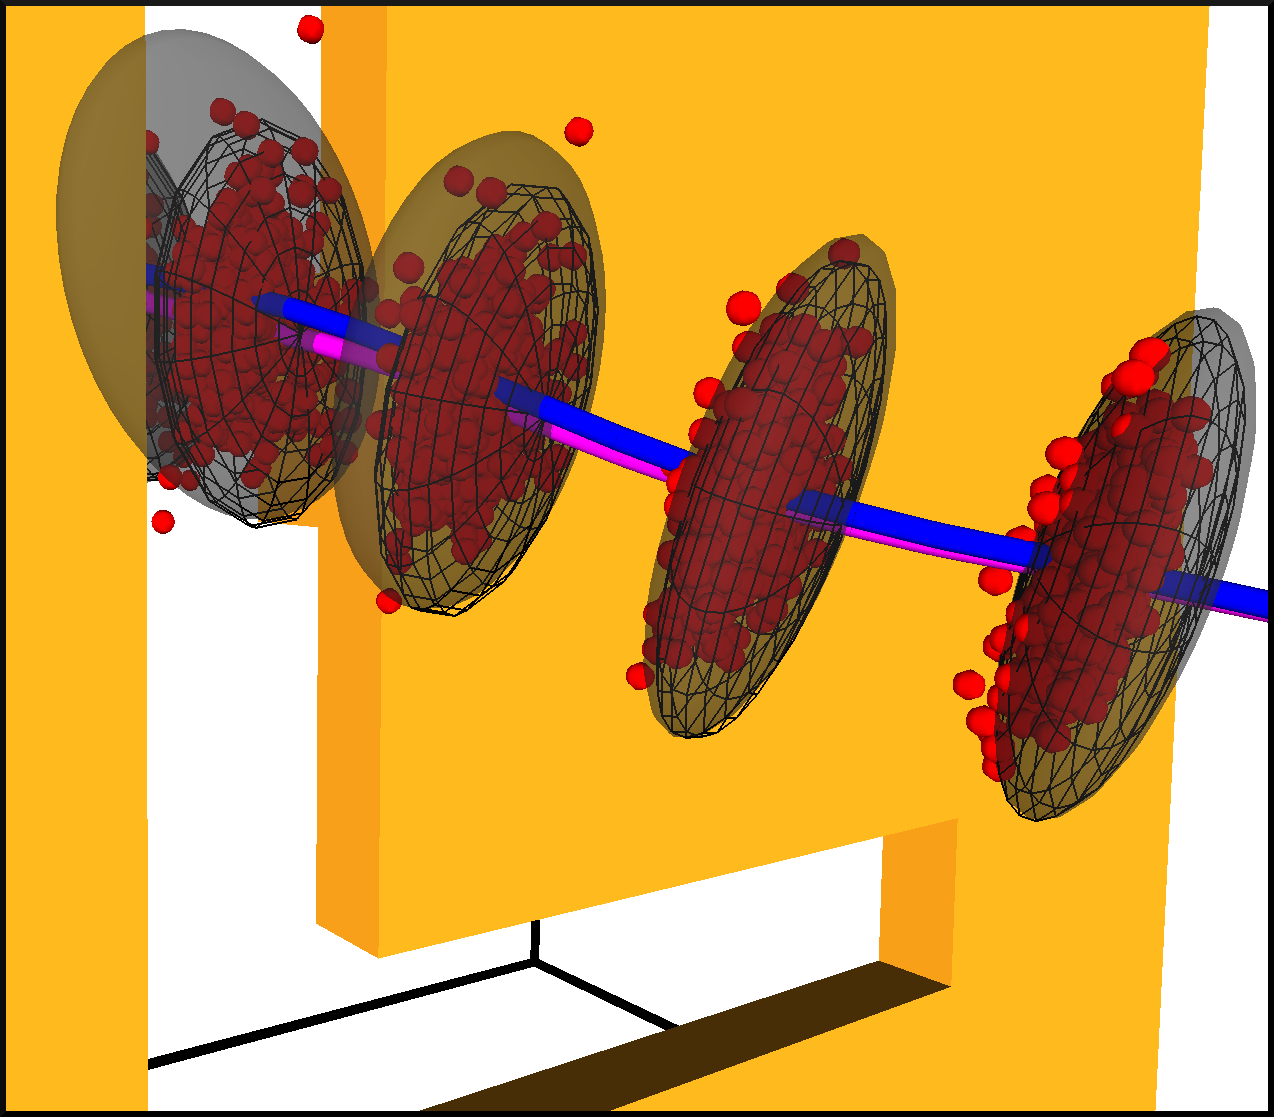
\includegraphics[width=100pt,clip]{figures/needle3d/plan1-closeup.png}}
\hfill
%\subfigure[Comparison with Monte Carlo simulations\label{fig:2d}]{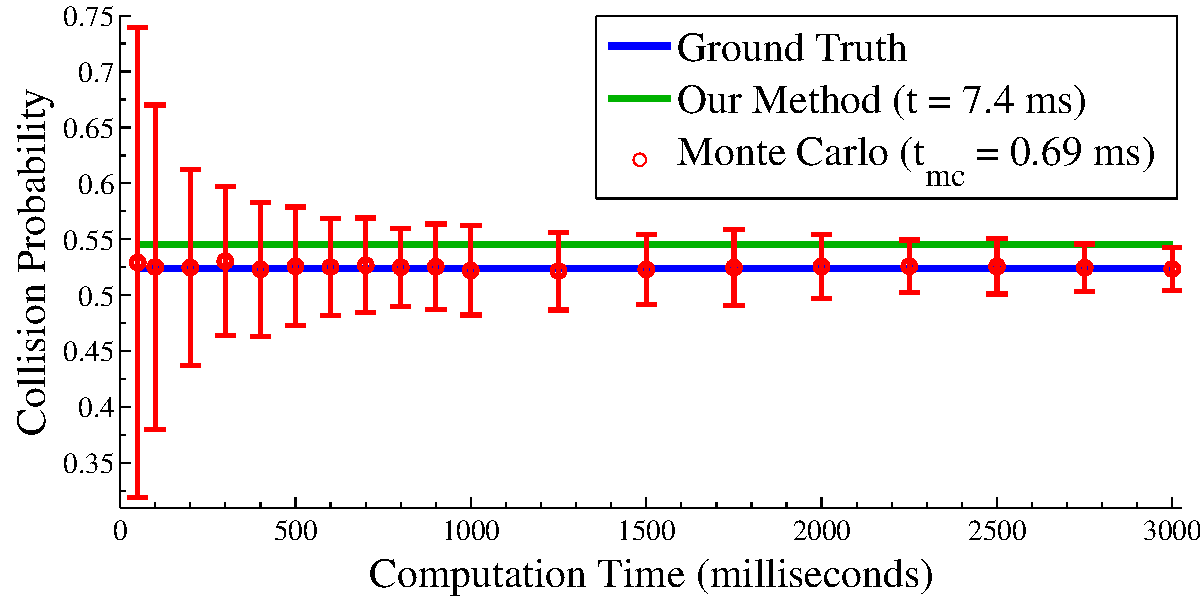
\includegraphics[width=180pt,clip]{figures/mc-needle.pdf}}
\subfigure[Comparison with Monte Carlo simulations\label{fig:2d}]{
\begin{overpic}[width=180pt,clip]{figures/mc-needle.pdf}
\put(27,5.1){\tiny $t_{mc}$}
\put(42.5,5.1){\tiny $t_{mc}$}
\put(57,5.1){\tiny $t_{mc}$}
\put(71.5,5.1){\tiny $t_{mc}$}
\put(86,5.1){\tiny $t_{mc}$}
\put(96,2.8){\tiny $t_{mc}$}
\end{overpic}}
\hfill
\subfigure[Different plan\label{fig:2c}]{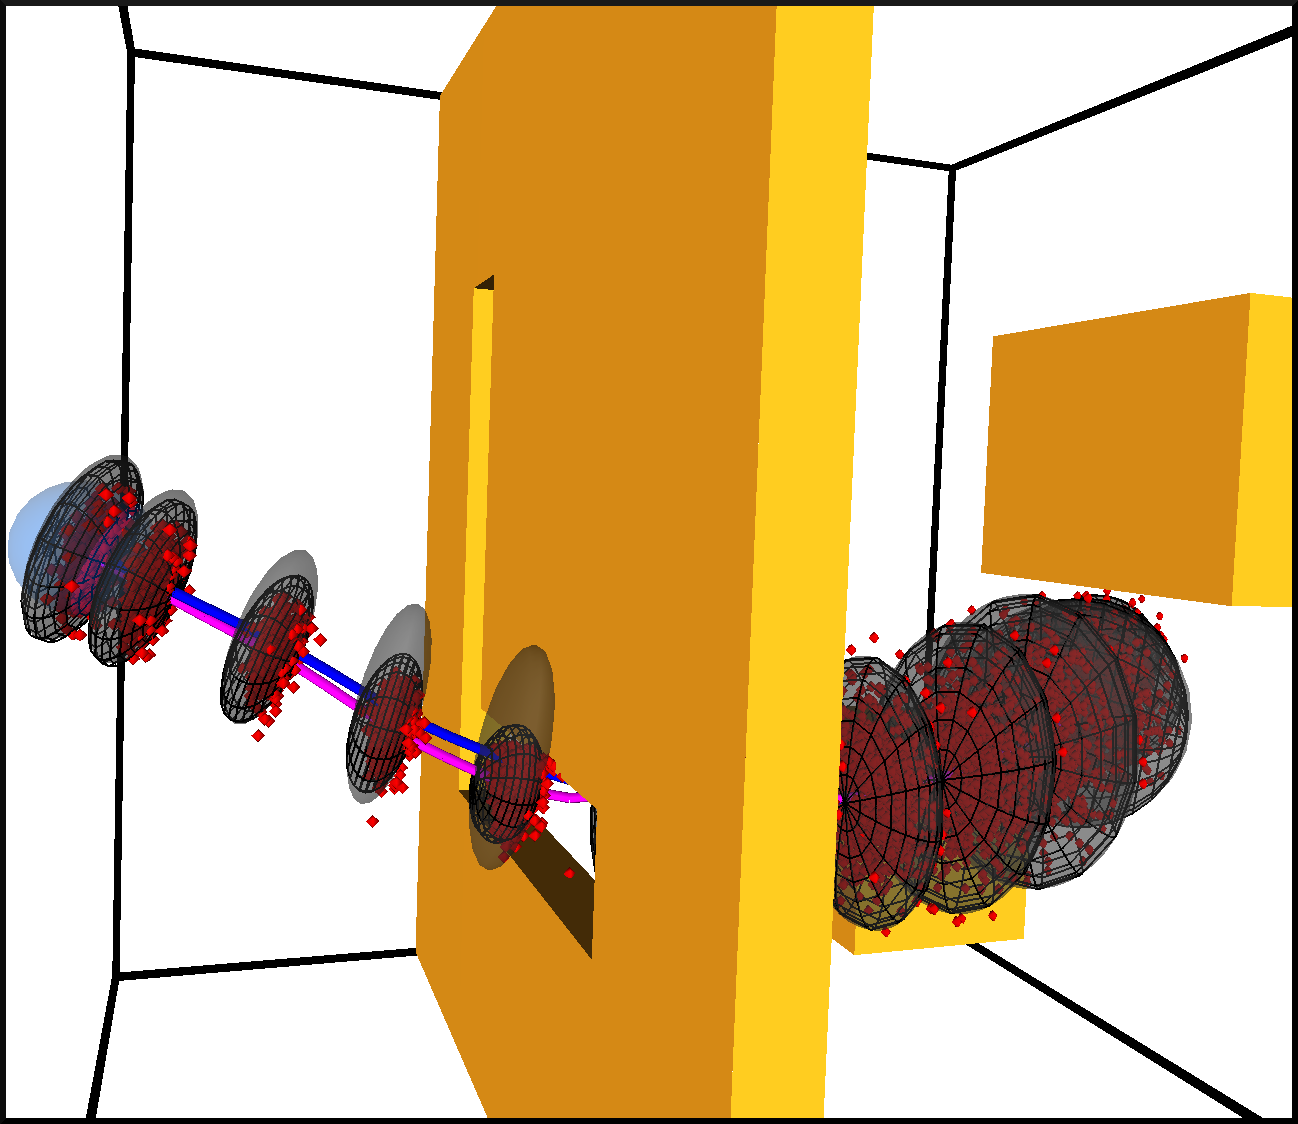
\includegraphics[width=100pt,clip]{figures/needle3d/plan2.png}}
{\,} \hfill
\vspace*{-5pt}
\caption{Nonholonomic bevel-tip steerable needle: (a) Unconditional distributions (solid gray ellipsoids corresponding to $3$ standard deviations) provide an overly conservative approximation of the uncertainty. Our method computes conditional distributions (black wireframe ellipsoids), which provide an accurate estimate of the probability distributions of the feasible robot states (shown in red). The collision probability estimated by our method is $54.5\%$, while the ground truth probability is $52.4\%$. (b) Zoomed in view of the conditional distributions in the narrow corridor. (c) Comparison of our method to Monte Carlo simulations. (d) The probability of collision estimated by our method for a second plan is $43.9\%$, while the ground truth probability is $42.2\%$.}
\vspace*{-15pt}
\label{fig:needle3d}
\end{figure*}

We also apply our method to a nonholonomic bevel-tip flexible needle \cite{Cowan2011_Chapter}, navigating in a 3D environment with obstacles (Fig.\ \ref{fig:2a}). This class of needles offers improved mobility,
enabling access to previously inaccessible targets while maneuvering around sensitive or impenetrable areas.

The state of the needle $\mathbf{x}$, is described by the $4 \times 4$ matrix $X = \left[\begin{smallmatrix} R & \mathbf{p} \\ \mathbf{0} & 1 \end{smallmatrix} \right] \in SE(3)$, where $\mathbf{p} \in \mathbb{R}^3$ is the position of the needle tip and $R \in SO(3)$ is the rotation matrix that encodes the orientation of the needle tip relative to a world coordinate frame. The needle naturally moves along constant curvature paths when inserted into tissue, but the curvature of the needle motion can be varied by duty cycled spinning of the needle during insertion. Under these modeling assumptions \cite{vandenBerg10_WAFR}, the control input $\mathbf{u} = [v, w, \kappa]^T \in \mathbb{R}^3$, consists of the insertion speed $v$, rotation speed applied at the base of the needle $w$, and the curvature $\kappa$.

It is convenient to describe the dynamics of the needle tip in terms of the instantaneous twist $U \in se(3)$ expressed in a local coordinate frame attached to the needle tip, given by:
\begin{equation}
U = \begin{bmatrix} [\mathbf{w}] & \mathbf{v} \\ \mathbf{0} & 0 \end{bmatrix}, ~ \mathbf{w} = \begin{bmatrix} v\kappa & 0 & w \end{bmatrix}^T, ~ \mathbf{v} = \begin{bmatrix} 0 & 0 & v \end{bmatrix}^T,
\end{equation}
where the notation $[\mathbf{s}]$ for a vector $\mathbf{s} \in \mathbb{R}^3$ refers to the $3 \times 3$ skew-symmetric cross-product matrix. The instantaneous twist $\tilde{U}$ that encodes the additive motion noise $\mathbf{m} = [\tilde{\mathbf{v}}^T ~ \tilde{\mathbf{w}}^T]^T \sim  \mathcal{N}[\mathbf{0}, M]$, can be similarly expressed.

Given a time step $\tau$, the stochastic discrete-time dynamics of the needle tip is given by the following model:
\begin{equation}
\mathbf{f}[\mathbf{x}, \mathbf{u}, \mathbf{m}] = X\exp(\tau (U + \tilde{U})).
\end{equation}

We also assume that we receive partial, noisy feedback on only the position of the needle tip $\mathbf{p}$, and not its orientation. This is a reasonable assumption since current medical imaging
technologies such as ultrasound do not allow for measuring the full state of the needle tip (as the imaging resolution is often too low to infer its orientation). The noise in the
sensor measurement is modeled as $\mathbf{n} \sim \mathcal{N}[\mathbf{0}, N]$. This gives the following stochastic measurement model:
\begin{equation}
\mathbf{h}[\mathbf{x}, \mathbf{n}] = \mathbf{p} + \mathbf{n}.
\end{equation}
We follow the approach in \cite{vandenBerg10_WAFR} to approximate the given nonlinear dynamics and measurement models with local linearizations around the nominal plan.

%Fig.\ \ref{fig:2b} shows the discrepancy between the unconditional and conditional distributions in the presence of obstacles. The conditional distributions computed using our method provide an accurate estimate of the distribution of the collision free robot states along the plan, thus providing an accurate estimate of the probability of collision.

\subsection{Analysis}

%\begin{figure}[!hbt]
%{\,} \hfill
%\subfigure[Car \label{fig:3a}]{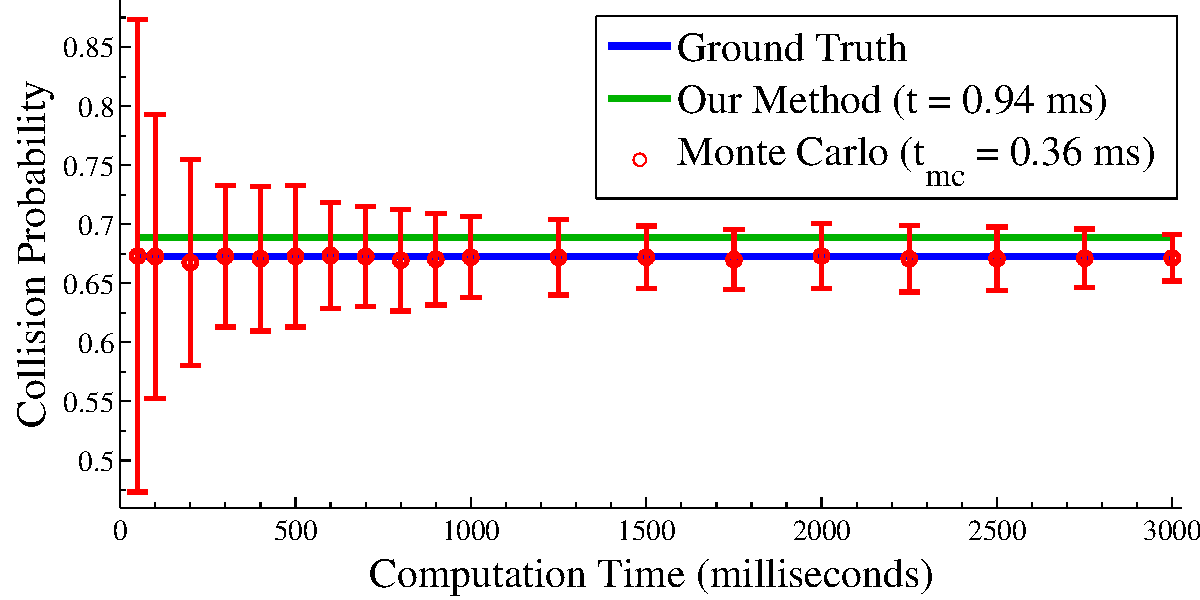
\includegraphics[width=120pt,clip]{figures/mc-car.pdf}}
%\hfill
%\subfigure[Needle \label{fig:3b}]{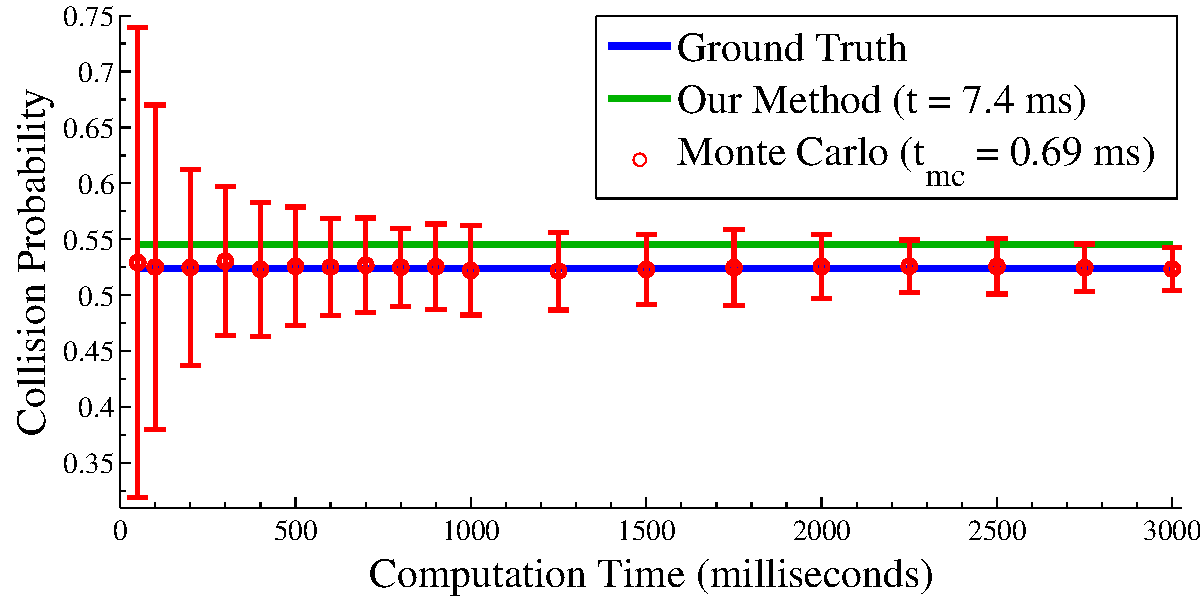
\includegraphics[width=120pt,clip]{figures/mc-needle.pdf}}
%{\,} \hfill
%\vspace*{-5pt}
%\caption{(a) XXX (b) YYY}
%\vspace*{-15pt}
%\label{fig:mcplots}
%\end{figure}

Table~\ref{tab:comp} compares the probability of collision estimated by our method against the ground truth probability computed using Monte Carlo simulations for the scenarios considered above. Our estimate lies within $5\%$ of the ground truth value. It is important to note that Monte Carlo simulations provide an unbiased estimate of the probability of collision, and can underestimate the probability if a sufficiently large number of samples are not considered. In contrast, our method provides a conservative estimate of the probability.

For the test case depicted in Fig.\ \ref{fig:1a}, each Monte Carlo simulation takes $0.36$ milliseconds, while our method requires a total computation time of $0.94$ milliseconds. Fig.\ \ref{fig:1d} shows the deviation in the probability estimates computed using Monte Carlo simulations with much fewer samples (computed over $100$ trials). As expected, the variance decreases as the number of Monte Carlo simulations increases. Even neglecting the fact that Monte Carlo simulations underestimate the collision probability, it still takes $3000$ simulations to arrive within the accuracy bounds of our method. This corresponds to over a second of computation time just to estimate the collision probability, which is undesirable for real-time motion planning under uncertainty.

Similarly, for the test case considered in Fig.\ \ref{fig:2a}, each Monte Carlo simulation takes $0.69$ milliseconds while our method takes $7.4$ milliseconds. It takes $2000$ simulations to arrive within the accuracy bounds of our method (Fig.\ \ref{fig:2d}), which corresponds to $1.4$ seconds of computation time. Our method provides accurate, yet conservative, estimates of the collision probability while incurring negligible computational overhead. This makes it especially suitable for online planning algorithms that explicitly consider uncertainty.

We compare our method to prior methods that rely on \emph{a priori} state distributions to estimate the collision probability. We generated a set of $100$ plans using the RRT planner using randomly initialized start states. For each plan, we estimated the collision probability using our method, applying Boole's inequality to the unconditional distributions \cite{Vitus11_ICRA}, and LQG-MP \cite{vandenBerg11_IJRR}. We use the mean error as a metric to compare the probability estimates to the ground truth probability. As summarized in Table~\ref{tab:comp}, the estimate computing using our method reduces the estimation error by more than $25\%$ as compared to the collision quality metric provided by LQG-MP \cite{vandenBerg11_IJRR} and the collision probability computed using the unconditional distributions directly \cite{Vitus11_ICRA}. It is important to note that all these estimation methods, including ours, provide a conservative bound for the collision probability.

\setlength{\tabcolsep}{1.5pt}
\begin{table}[bht]
\centering
        \resizebox{3.4in}{!}{
        \begin{tabular}{|c||c|c||c|c||c|c|}
                \hline
                Robot & \multicolumn{2}{|c||}{Our method} &\multicolumn{2}{|c||}{Unconditional \cite{Vitus11_ICRA}}   &\multicolumn{2}{|c|}{LQG-MP \cite{vandenBerg11_IJRR}} \\
                \hline
                &MAE    &Avg. Time   &MAE        &Avg. Time   &MAE      &Avg. Time\\
                &(\%)   &(ms) &(\%)   &(ms) &(\%) &(ms)\\
                %&MAE (\%) &Time (ms) &MAE (\%) &Time (ms)  &MAE (\%) &Time (ms)\\
                \hline
                %& & & & & &\\
                car & 3.0 ($\pm$ 2) & 9 & 28.0 ($\pm$ 15) & 6 & 52.2 ($\pm$ 15) & 4 \\
                %&($\pm$ 1.9) & &($\pm$ 15.1) & &($\pm$ 15.4) &\\
                \hline
                %& & & & & &\\
                needle & 5.0 ($\pm$ 3) & 14 & 20.7 ($\pm$ 7) & 12 & 61.7 ($\pm$ 12) & 10\\
                %&($\pm$ 3.0)& & ($\pm$ 6.9) & & ($\pm$ 11.5) &\\
                \hline
        \end{tabular}
        }
        \caption{Comparison of our method with prior methods over $100$ plans in terms of mean absolute error (MAE) from ground truth probability. Standard deviations provided in parentheses.}
        \label{tab:comp}
%\vspace{-15pt}
\vspace{-20pt}
\end{table}
